
\clearpage









\section{Abstract}

The third chapter of my thesis.
Basically the same as the second.




%%%%%%%%%%%%%%%%%%%%%%%%%%%%%%%%%%%%%%%%%%%%%%%%%%%%%%%%%%%%%%%%%%%%%%%%%%%%%%%%%%%%%%%%%%%%%%%%%%%%%%%%%%%%%%%%%%%%%%%%%%%%%%%%%%%%%%%%%%%%%%%%%%%%%%%%%%%

\section{Introduction}

%%%%%%%%%%%%%%%%%%%%%%%%%%%%%%%%%%%%%%%%%%%%%%%%%%%%%%%%%%%%%%%%%%%%%%%%%%%%%%%%%%%%%%%%%%%%%%%%%%%%%%%%%%%%%%%%%%%%%%%%%%%%%%%%%%%%%%%%%%%%%%%%%%%%%%%%%%%

More text.


\section{Methods}

Here I describe my methods interspersed with the code that actually does it.











\begin{knitrout}\footnotesize
\definecolor{shadecolor}{rgb}{0.969, 0.969, 0.969}\color{fgcolor}\begin{figure}[t]

{\centering 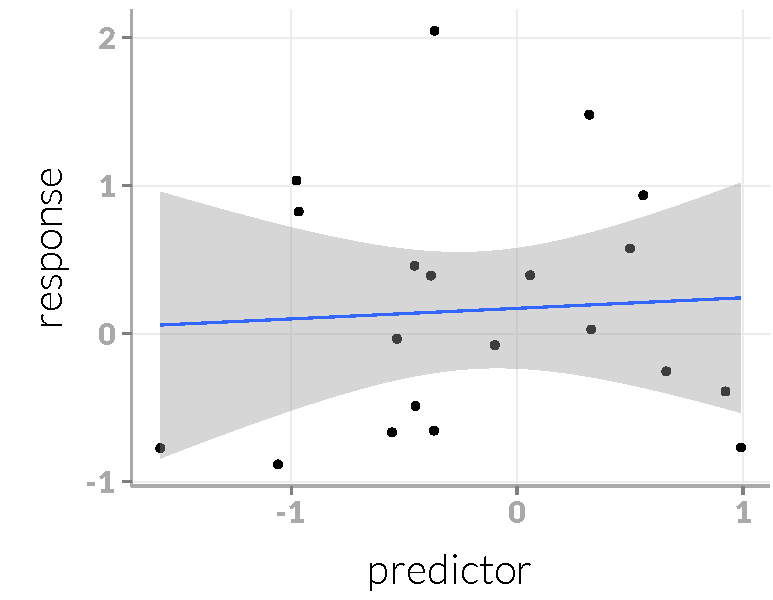
\includegraphics[width=0.8\textwidth]{figure/figPlots-1} 

}

\caption[A great figure.]{
Caption labels can be really long so they might want to be separate. 
}\label{f:figPlots}
\end{figure}


\end{knitrout}

\section{Methods}

Remember to put results directly into text with \texttt{\\rinline}.
My model for this chapter is also poor (p = 0.32).

